\chapter{Modélisation des séquences d'opérations des deux pièces}
Dans cette partie, l'objet de l'étude se porte sur la réalisation de 6 opérations, 3 par pièces (les opérations $o_1 , o_3 , o_5$ pour $p_1$ et $o_2 , o_4 , o_6 $ pour $p_2$). Il faut, dans un premier temps, trouver une séquence optimale telle que toutes les opérations soient effectuées en un temps minimum sans déclencher l'alarme. Ensuite, nous devons réaliser une commande en réseau de Petri temporel pour effectuer les opérations puis l'analyser à l'aide d'un graphe des classes. Dans un dernier temps, nous avons réaliser la commande en langage C. 
\section{Analyse d'ordonnancement}
Nous avons décidé d'étudier l'ordonnancement optimal par un chronogramme car nous avons trouvé l'approche graphique plus intuitive au vu du faible nombre d'opérations. Nous avons réalisé cet ordonnancement sur Excel en prenant pour échelle \emph{une case égale une seconde}. Le chronogramme (figure \ref{fig:ordoExcel}) est coupé en trois parties pour des raisons de visibilité : une ligne est réservée aux opérations liées à la pièce $p_2$, une seconde aux actions du charriot et une dernière aux opérations de $p_1$.

\begin{figure}[!ht]
\centering
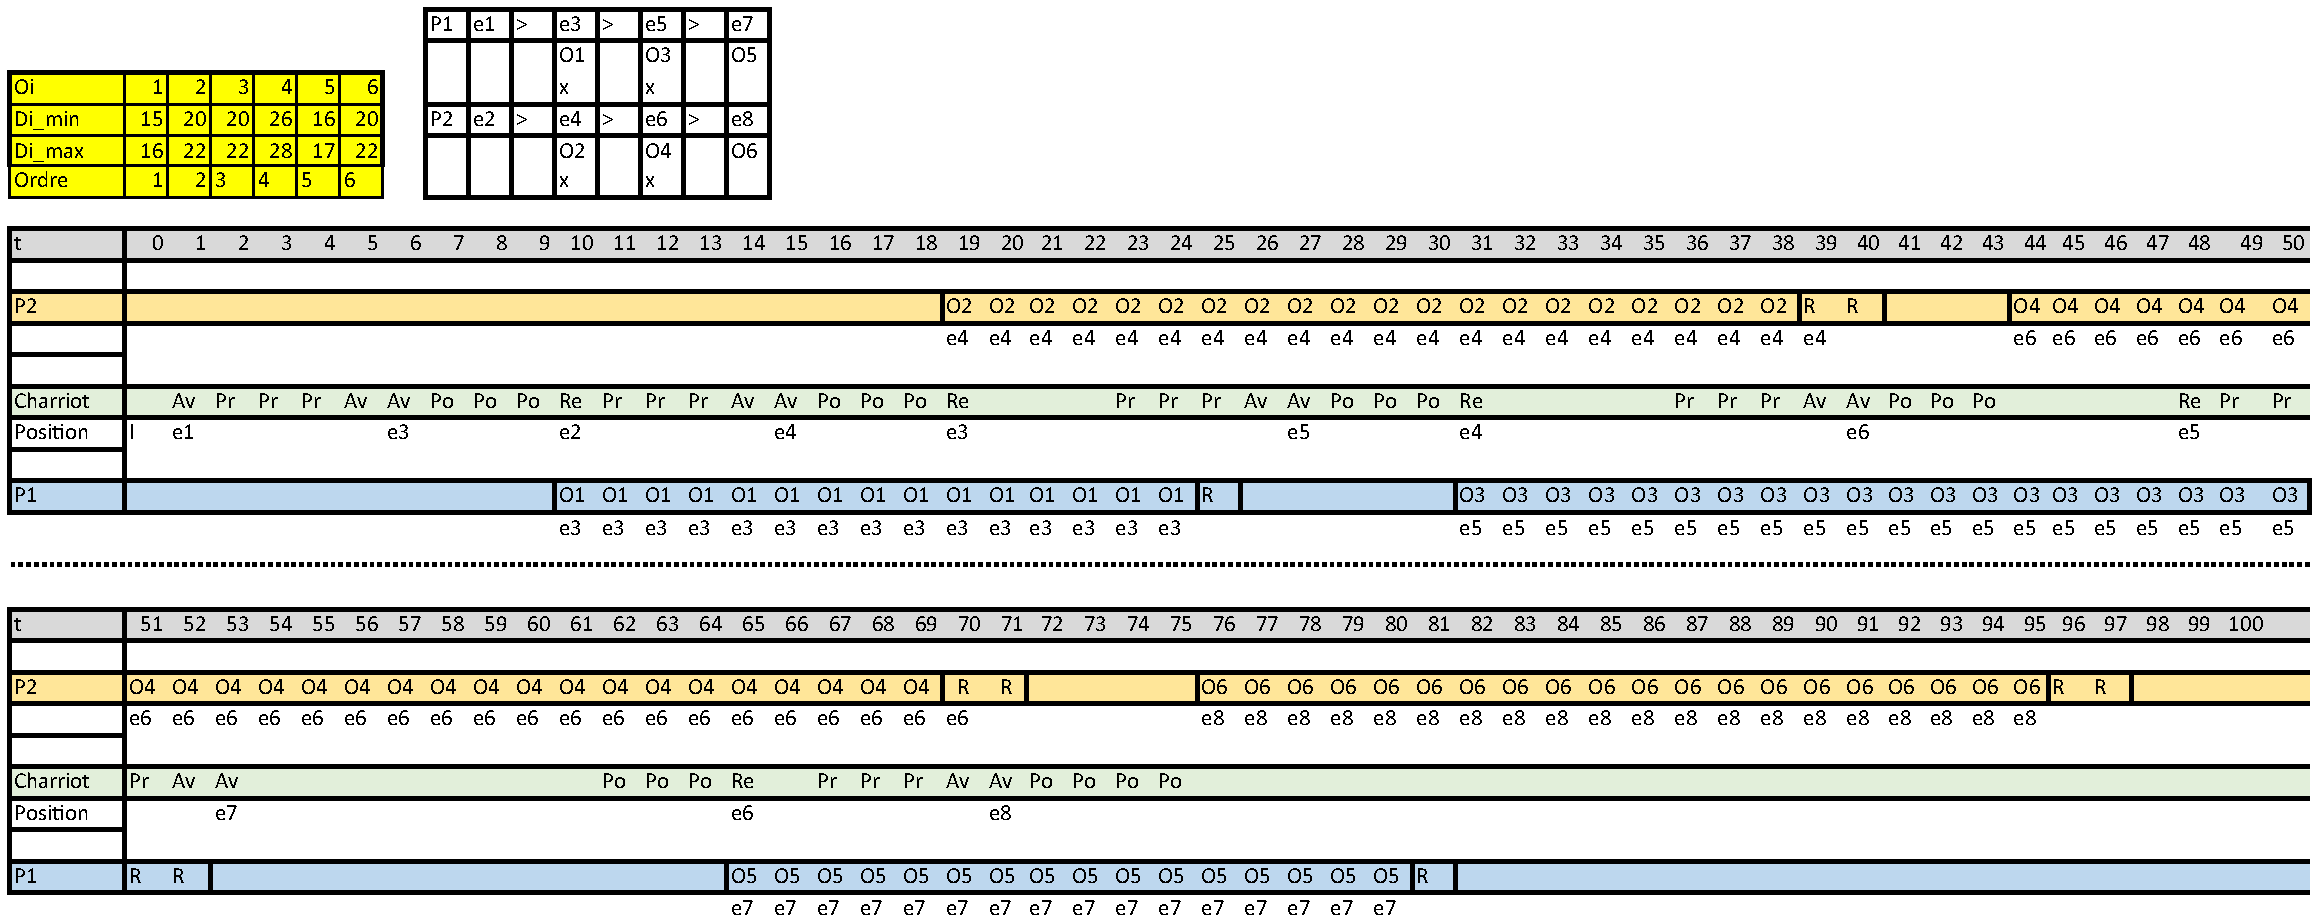
\includegraphics[width=\textwidth]{./III/images/ordo.pdf}
\caption{\label{fig:ordoExcel}Capture du tableur de calcul de l'ordonnancement.}
\end{figure}

Nous avons positionné les opérations au plus tôt, en vérifiant qu'elles n'empêchent pas de récupérer les pièces avant leurs alarmes respectives. Par exemple, l'opération $o_5$ pourrait commencer à partir de la 57\ieme seconde mais il serait impossible de retirer les deux pièces avant leurs alarmes donc nous avons décalé $o_5$ de façon à ce que, ni la pose, ni la prise de la pièce $p_1$ ne perturbe la prise et la pose de $p_2$. De plus, nous prenons pour hypothèse que les deux dernières opérations $o_5$ et $o_6$ n'ont pas de date récupération maximale et peuvent rester respectivement en $e_7$ et en $e_8$ car ces deux emplacements représentant le bac de sortie. Si nous avions pris le partie de les ramener à leurs emplacements initiaux, cela n'aurait pas été possible avec l'ordonnancement actuel, il aurait fallu organiser les opérations différemment de façon à avoir le temps de ramener les pièces au début ce qui nécessite beaucoup de temps à cause de la distance de déplacement importante.

\section{Réseau de Petri de commande}
Nous avons transformer la séquence d'actions de la ligne \emph{Chariot} de l'ordonnancement précédent (voir figure \ref{fig:ordoExcel}) en un réseau de Petri temporel. À chaque fois que le charriot dépose une pièce, on lance un
\section{Analyse par graphe de classes}

\section{Implémentation}